\documentclass[a4paper,12pt]{article} % тип документа

\usepackage{tikz}
\usepackage[T2A]{fontenc}			% кодировка
\usepackage[utf8]{inputenc}			% кодировка исходного текста
\usepackage[english,russian]{babel}	% локализация и переносы
\usepackage{amsfonts,longtable}

% Математика
\usepackage{amsmath,amsfonts,amssymb,amsthm,mathtools} 


\usepackage{wasysym}

\title{Лабораторная работа 1.3.1 по курсу \\ "Общая физика"  \\ 
\vspace{0.2cm}
\vspace{4.5cm}
 \LARGE{\textbf{Определение модуля Юнга на основе исследования деформаций растяжения и изгиба}}\vspace{5.5cm}}
\date{09.11.2018}
\usepackage{tikz}
\author{\vspace{0.2cm}Баринов Леонид}

\begin{document}
\maketitle
\newpage
\section{Аннотация}
В работе будет экспериментально получена зависимость между напряжением и деформацией для двух простеших напряженных состояний упругих тел: одноосного растяжения и чистого изгиба; по результатам измерений будет определен модуль Юнга и его погрешность.
\section{Теоритические сведения}
На Рис. 1а показана балка, деформированная под действием силы $P$, приложенной поссредине между опопрами А и Б. Со стороны опор на балку в точках А и Б действуют силы $P/2$. Деформация балки проиходит таким образом, что продольные слои в верзней ее части оказываются сжатыми, а в нижней -- растянутыми. Можно считать, что абсолютные величины напряжений по слоям растут пропорционально расстоянию от середней линнии балки, как показано стрелками на Рис. 1б для выделенного элемента балки. Так как средняя часть элемента не напряжена, то длина средней линии элемента $dl_0$ при деформации не меняется (так же, как длина средней линии всей балки). Такое напряженное состояние балки называется чистым изгибом. Считаема, что напряжения в слоях связаны с их деформацией законом Гука:
\begin{equation}
\sigma = E\frac{dl - dl_0}{dl_0}
\end{equation}
В выделенном на рис. 1в элементе балки наклон средней линии на ее длине $dl_0$ меняется от $\alpha$ до $\alpha-d\alpha$. Длину дуги можно выразить через радиус ее кривизны $R$:
\begin{equation}
dl_0 = -Rd\alpha
\end{equation}
Знак минус здесь потому, что $R$ мы считаем положительным, а угол наклона средней линии балки в вырбранных на Рис. 1а координатах уменьшается по длине балки (как это показано на Рис. 1в). Если $y(x)$ -- зависимость, описывающая форму средней линии балки в выбранной системе координат $x, y$, то угол наклона средней линии определяется выражением
\begin{equation}
\frac{dy(x)}{dx} = \tg\alpha
\end{equation}
Длину средней линии малого элемента балки можно выразить следующим образом (см. Рис. 1г):
\begin{equation}
dl_0 = \sqrt{(dx)^2+(dy)^2} = dx\sqrt{1 + \left(\frac{dy}{dx}\right)^2}
\end{equation}
\newpage
\begin{figure}[h]
\centering
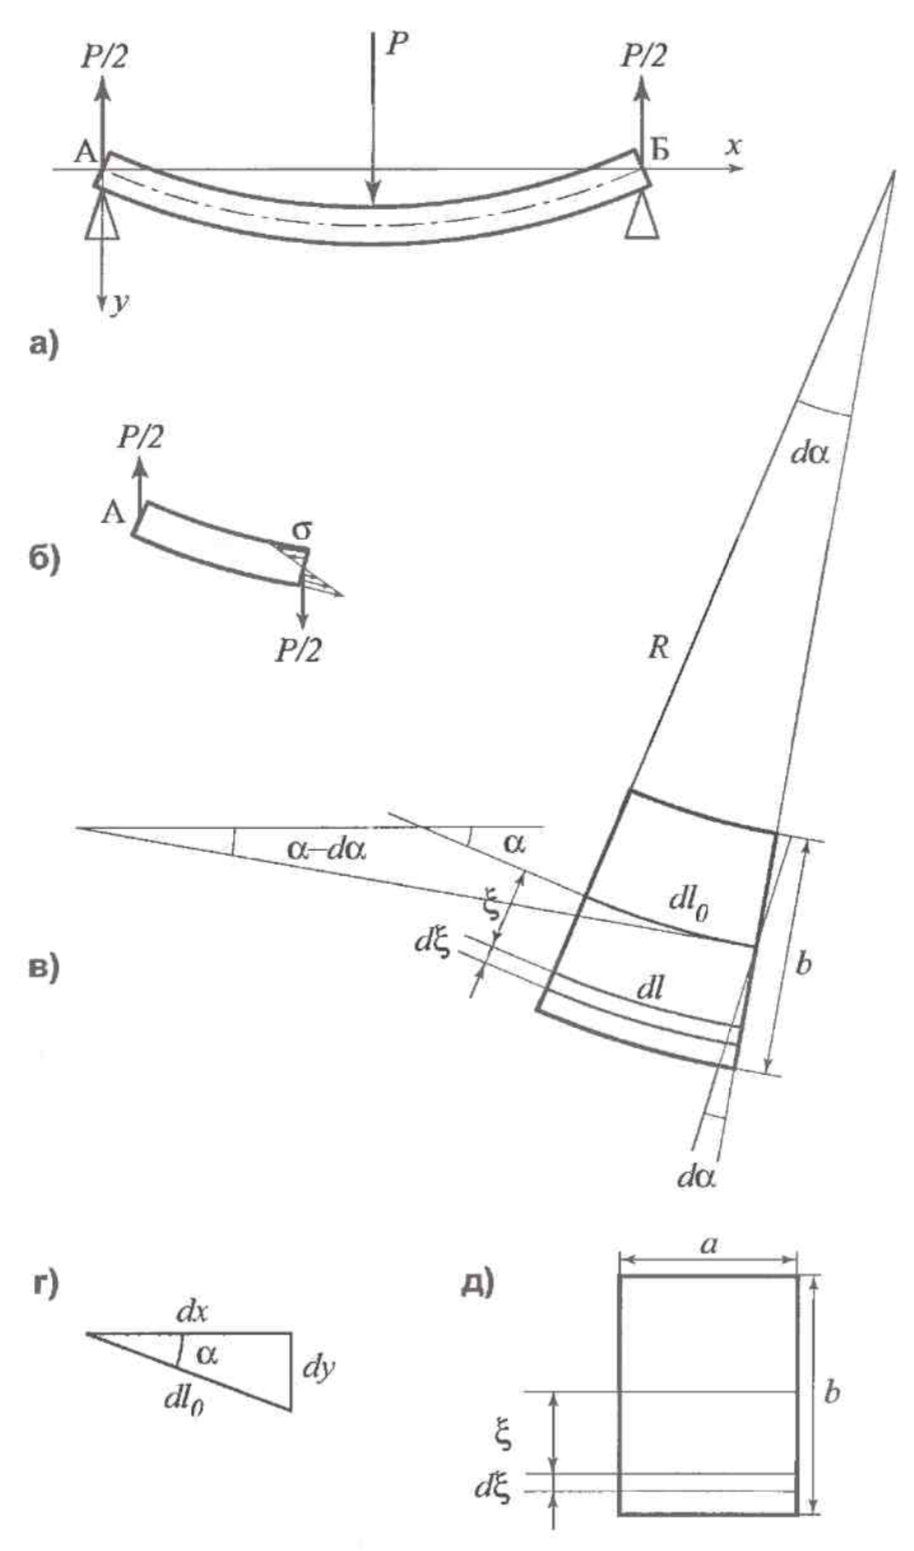
\includegraphics[scale=0.5]{3}
\caption{Изгиб балки}
\end{figure}
Из этого же треугольника 
\begin{equation}
\frac{dx}{dl_0} = \cos\alpha
\end{equation}
Дифференцируя (3) по $x$ и пользуясь (2), получаем
\begin{equation}
\frac{d^2y}{dx^2} = \frac{1}{\cos^2\alpha}\frac{d\alpha}{dx} = \left(\frac{dl_0}{dx}\right)^2 \frac{d\alpha}{dl_0}\frac{dl_0}{dx} = - \left(\frac{dl_0}{dx}\right)^3\frac{1}{R}
\end{equation}
Отсюда и из (4) следует
\begin{equation}
\frac{1}{R} = -\frac{y''}{(1+y'^2)^{3/2}}
\end{equation}
Напряжение в продольном слое, находящемся на расстоянии $\xi$ от средней линии балки (см. Рис. 1в) и описываемое формулой (1), можно представить следующим образом:
\begin{equation}
\sigma = E\frac{dl - dl_0}{dl_0} = \frac{E}{R}\xi
\end{equation}
Здесь использовано соотношение, следующее из подобия тругольников наРис. 1в:
\begin{equation}
\frac{dl-dl_0}{\xi} = \frac{dl_0}{R}
\end{equation}
Сумма сил упругости, действующих в сечении балки, равна нулю, поэтому их суммарный момент не зависит от положения точки, относительно которой огн вычисляется. Выберем эту точку на средней линии балки. Получаем:
\begin{equation}
M = \int\limits_{-b/2}^{b/2} \xi\sigma d S = \frac{E}{R}\int\limits_{-b/2}^{b/2}\xi^2 d S = \frac{E}{R}I
\end{equation}
где $dS = as\xi$, $a$ -- ширина, $b$ -- высота поперечного сечения балки (см. Рис 1д). $I$ называют моментом инерции поперечного сечения балки относительно оси, проходящей через срденюю линию балки. Из Рис. 3б видно, что для части балки (от $x = 0$ до $x$) равновесие обеспечивается равенством сил, приложенных в точке опоры и в рассамтриваемом сечении, а также равенством моментов этих сил и момента, определяемого формулой (10).\\
Равенсто моментов дает
\begin{equation}
\frac{El}{R} = \frac{xP}{2}
\end{equation}
Теперь, используя (7), можно написать уравнение, определяющее форму средней линии балки:
\begin{equation}
y'' = -(1+y'^2)^{3/2}\frac{P}{2EI}x
\end{equation}
При малых прогибах
\begin{equation}
y'^2 \ll 1
\end{equation}
В этом случае из (12) следует
\begin{equation}
y'' = -\frac{P}{2EI}x
\end{equation}
Интегрируя это уравнение, получаем
\begin{equation}
y' = -\frac{P}{4EI}x^2 + C
\end{equation}
Здесь $C$ -- постоянная, которая определяется из условия симметрии прогиба $y' = 0$ при $x = l/2$. Из (15) следует
\begin{equation}
y' = - \frac{P}{4EI}\left(x^2-\frac{l^2}{4}\right)
\end{equation}
Интегрируя еще раз и учитывая, что при $x = 0$ также и $y = 0$, получаем уравнение средней линии балки:
\begin{equation}
y = \frac{Px}{48EI}(3l^2-4x^2)
\end{equation}
Максимальный прогиб балки, который определяется величиной $y$ при $x = l/2$, равен
\begin{equation}
y_{max} = \frac{Pl^3}{48EI}
\end{equation}
В случае прямоугольного сечения балки 
\begin{equation}
I = \int\limits_{-b/2}^{b/2}\xi^2 d S = a\int\limits_{-b/2}^{b/2}\xi^2d\xi = \frac{ab^3}{12}
\end{equation}
Из (18) и (19) для модуля Юнга получаем
\begin{equation}
E = \frac{Pl^3}{4ab^3y_{max}}
\end{equation}
\section{Оборудование и инструментальные погрешности}
В первой части работы производим растяжение проволки, и это соответсвует случаю одноосного напряженного состояния, описываемого форумлой 
\[\sigma = E\varepsilon\]
$\sigma$ - напряжение\\
$E$ - модуль Юнга\\
Во второй части работы измерения производят при изгибе балки, которую иногда будем называть бруском, а иногда -- стержнем. Связь между прогибом балки и величиной силы, приложенной посредине между точками опор балки, может быть выражена через модуль Юнга. Это позволяет по измерениям приложенных сил и прогиба определить модуль Юнга.\\
\textbf{Установка 1}\\
Диаметр проволки:
\[d = 0,46\text{мм}\]
Длина рычага:
\[r = 15\text{мм}\]
Расстояние от шкалы до зеркала:
\[h = 138\text{см}\]
\[\sigma_h = 0,5\text{см}\]
Длина проволки:
\[l = 176\text{см}\]
\[\sigma_l = 0,5\text{см}\]
\textbf{Установка 2}\\
Расстояние между ребрами призм A и Б
\[l_\text{АБ} = 50\text{см}\]
\[\sigma_{l_\text{АБ}} = 0,1\text{см}\]
Погрешность измерения штангенциркулем:
\[\sigma = 0,1\text{мм}\]
\section{Эксперементальные установки}
\subsection{Определение модуля Юнга по измерениям растяжения проволки}
Для определения модуля Юнга используется прибор Лермантова, схема которого изображена на Рис. 2. Верхний конец проволки П, изготовленной из исследуемого материала, прикреплен к консоли К, а нижний -- к цилиндру, которым оканчивается шарнирный кронштейн Ш. На этот же цилиндр опирается рычаг $r$, связанный с зеркальцем З. Таким образом, удлинение проволоки можно измерить по углу поворота зеркальца.

Натяжение проволоки можно менять, перекладывая грузы с площадки М на площадку О и наоборот. Такая система позволяет исключить влияние деформации кронштейна К на точность изерений, так как нагрузка на нем все время остается постоянной.

При проведении эксперимента следует иметь в виду, что проволока П при отсутствии нагрузки всегда несколько изогнута, что не может не сказываться на результатах, особенно при небольших нагрузках. Проволока вначале не столько растягивается, сколько распрямляется.

Выведем формулу, связывающую число делений по шкале $n$, расстояние $h$ от шкалы до зеркальца, длину рычага $r$ и удлинение проволки $\Delta l$
\[\tg\varphi = \frac{\Delta l}{r}\]
$\varphi$ - угол поворота зеркальца
\[\tg 2\varphi = \frac{\Delta n}{n}\]
$\Delta n$ - расстояние между делениями, соответствующие повороту зеркальца на $\varphi$ и начальной нагрузке
В силу малости $\varphi$ $\tg 2\varphi \approx 2 \tg \varphi$
\[2\frac{\Delta l}{r} = \frac{\Delta n}{h}\]
\[\Delta l = \frac{\Delta n r}{2h}\]
\begin{figure}[!h]
\centering
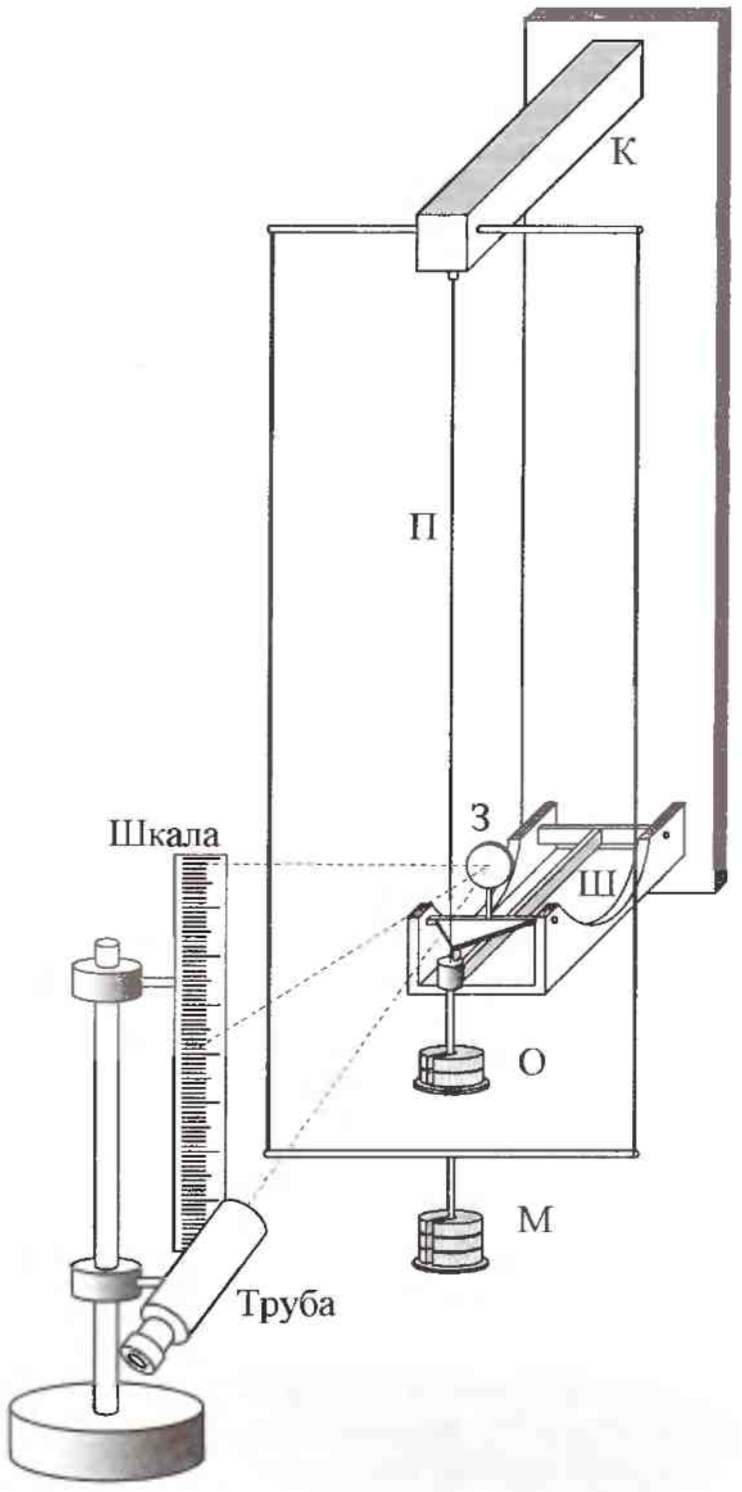
\includegraphics[scale=0.3]{1}
\caption{Прибор Лермантова}
\end{figure}
\newpage
\subsection{Определение модуля Юнга по измерениям изгиба балки}
Экспериментаьная установка состоит из прочной стойки с опорными призмами А и Б (Рис. 3). На ребра призм опирается исследуемный стержень (балка) В. В середине стержня на призме Д подвешена площадка П с грузами. Измерять стрелу прогиба можно с помощью индикатора И, укрепляемого на отдельной штанге. Полный оборот большой стрелки индикатора соответсвует 1 мм и одному делению малого цифирблата

\begin{figure}[h]
\centering
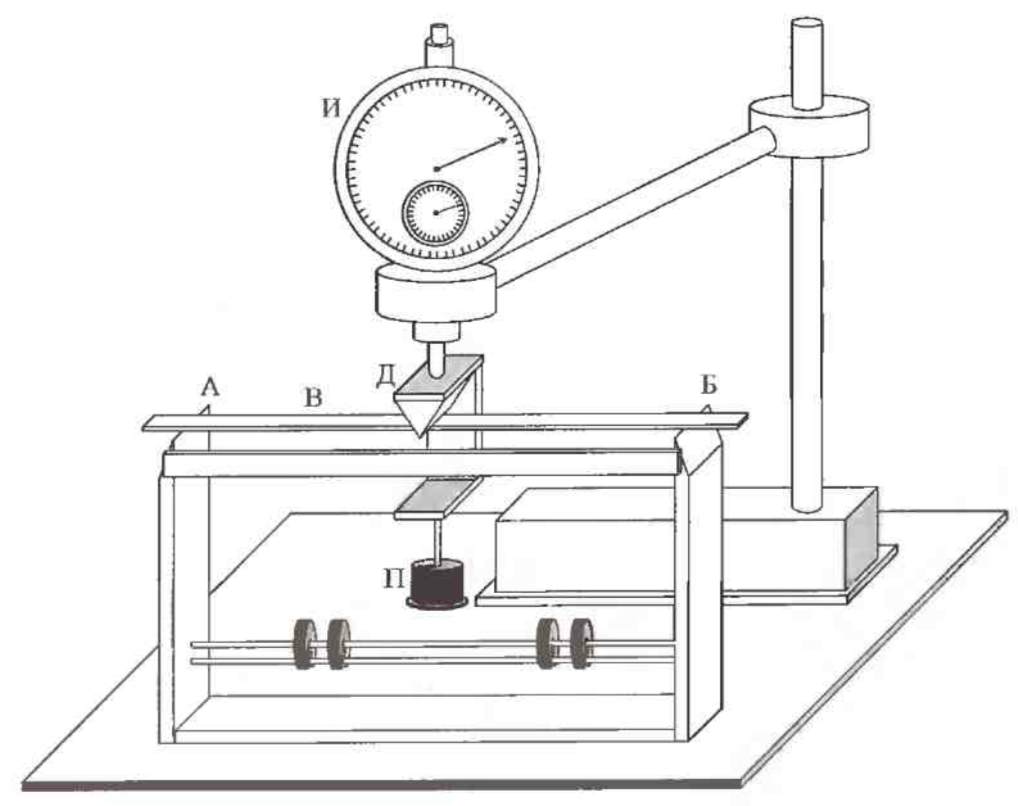
\includegraphics[scale=0.4]{2}
\caption{Схема установки для измерения модуля Юнга}
\end{figure}
Модуль Юнга $E$ материала стержня связан со стрелой прогиба $y_max$ (то есть с перемещением середины стержня) соотношением
\begin{equation}
 E = \frac{P l^3}{4ab^3y_{max}}
\end{equation}

Здесь $P$ -- нагрузка, вызывающая прогиб стержня, $l$ -расстояние между призмами А и Б, $a$ и $b$ -- ширина и высота сечения стержня.
\section{Результаты измерений и обработка результатов}
\subsection{Определение модуля Юнга по измерениям растяжения проволки}
Вычислим площадь поперечного сечения проволки:
\[S = \frac{1}{4}\pi d^2 = 0,17\text{мм}^2\]
Снимем зависимость удлинения проволки (число делений $n$ по шкале) от массы грузов $m$ при увелечении и уменьшении нагрузки. Без штриха указано удлинение проволки при нагрузки, со штрихом при разгрузке. $\Delta x, \Delta l, \sigma_{\Delta_l}$ указаны в $\text{мм}$
\begin{table}[h]
\centering
\begin{tabular}{|c|c|c|c|c|c|c|c|c|c|}
\hline
$m,\text{г} $   & $P, H$ & $\Delta x_1$   & $\Delta x'_1$  & $\Delta x_2,$   & $\Delta x'_2$  & $\Delta x_3$   & $\Delta x'_3$ & $\Delta l$ & $\sigma_{\Delta_l}$  \\ \hline
503,3  & 5,033  & 261 & 259 & 257 & 256 & 257 & 256 & 0      & 0      \\ \hline
985,8  & 9,858  & 294 & 293 & 291 & 291 & 291 & 291 & 0,1857 & 0,0037 \\ \hline
1489,3 & 14,893 & 341 & 340   & 338 & 339 & 338 & 338 & 0,4420 & 0,0051 \\ \hline
1952,9 & 19,529 & 395 & 393 & 392 & 392 & 391 & 392 & 0,7328 & 0,0049 \\ \hline
2408,2 & 24,082 & 453 & 451 & 451 & 450   & 450   & 450   & 1,0498 & 0,0049 \\ \hline
\end{tabular}
\caption{Зависимость удлинения проволки от массы грузов}
\end{table}
По данным Таблицы 1 построим график зависимости удлинения проволоки $\Delta l$ от нагрузки $P$. Аппроксимируем полседние четыре точки, так как при малых нагрузках удлинение проволоки определяется не растяжением, а выпрямлением.
\begin{figure}[h]
\centering
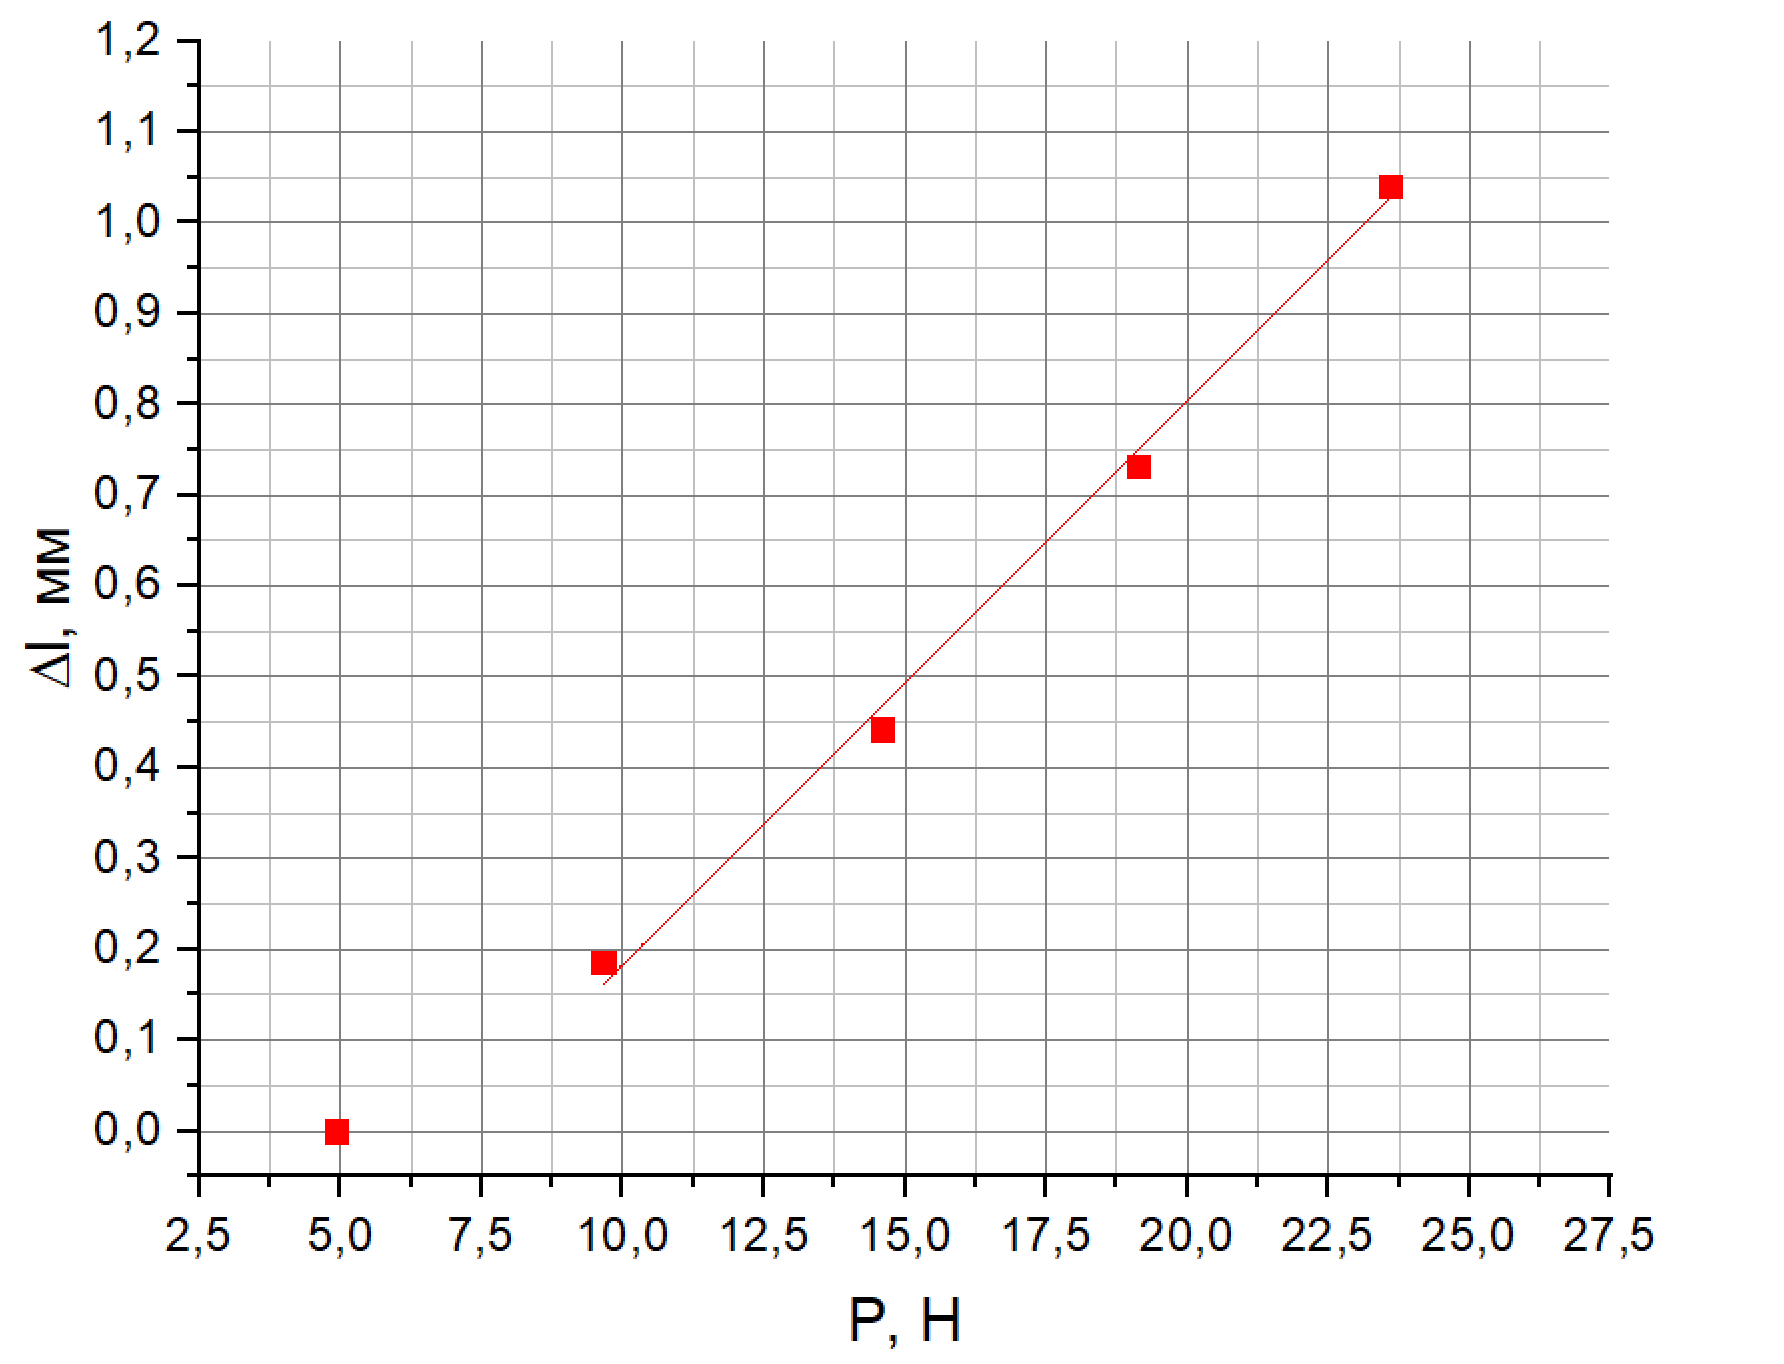
\includegraphics[scale=0.4]{5}
\caption{Зависимость удлинения проволоки $\Delta l$ от нагрузки $P$}
\end{figure}

По наклону графика определим жесткость проволки $k$
\[k = (16111\pm1048)\frac{\text{H}}{\text{м}}\]
Определим модуль Юнга по формуле:
\[E = \frac{kl_0}{S} = 16,7\cdot 10^{10}\frac{\text{Н}}{\text{м}^2}\]
Погрешность модуля Юнга приблизительно равна погрешности жесткости $k$, так как погрешность длины проволоки $l$ пренебрижимо мала
\[\sigma_E = 1\cdot 10^{10} \frac{\text{Н}}{\text{м}^2}\]
\subsection{Определение модуля Юнга по измерениям изгиба балки}
Определим ширину $a$ и толщину $b$ металлической и двух деревянных балок. Результаты занесем в Таблицы 2, 3, 4 соответсвенно.
\begin{table}[h]
\centering
\begin{tabular}{|c|c|c|c|c|c|c|c|c|c|c|}
\hline
$\text{№}$     & 1    & 2    & 3    & 4    & 5    & 6    & 7    & 8    & 9    & 10   \\ \hline
$a, \text{cм}$ & 2,15 & 2,17 & 2,15 & 2,17 & 2,16 & 2,15 & 2,16 & 2,15 & 2,15 & 2,17 \\ \hline
$b, \text{cм}$ & 0,4  & 0,4  & 0,39 & 0,4  & 0,41 & 0,4  & 0,4  & 0,39 & 0,4  & 0,4  \\ \hline
\end{tabular}
\caption{Ширина $a$ и толщина $b$ металлической балки}
\end{table}
\[a_{\text{ср}_1} =(2,158\pm0,01)\text{см} \]
\[b_{\text{ср}_1} =(0,040\pm0,01)\text{см} \]
\begin{table}[h]
\centering
\begin{tabular}{|c|c|c|c|c|c|c|c|c|c|c|}
\hline
$\text{№}$ & 1   & 2    & 3    & 4    & 5    & 6    & 7    & 8    & 9    & 10   \\ \hline
$a, \text{cм}$& 2   & 2,03 & 2,06 & 2,04 & 2,02 & 2,04 & 2,04 & 2,02 & 2,03 & 2,06 \\ \hline
$b, \text{cм}$ & 1,1 & 1,1  & 1,12 & 1,08 & 1,06 & 1,06 & 1,06 & 1,04 & 1,04 & 1    \\ \hline
\end{tabular}
\caption{Ширина $a$ и толщина $b$ первой деревянной балки}
\end{table}
\[a_{\text{ср}_2} =(2,03\pm0,02)\text{см} \]
\[b_{\text{ср}_2} =(1,07\pm0,03)\text{см} \]
\newpage
\begin{table}[h]
\centering
\begin{tabular}{|c|c|c|c|c|c|c|c|c|c|c|}
\hline
$\text{№}$ & 1    & 2    & 3    & 4    & 5    & 6    & 7    & 8    & 9    & 10   \\ \hline
$a, \text{cм}$ & 2,03 & 2,04 & 2,05 & 2,04 & 2,02 & 1,97 & 2,06 & 2,01 & 2,05 & 2,04 \\ \hline
$b, \text{cм}$ & 1,02 & 1,05 & 1,02 & 1,03 & 1,02 & 1,03 & 1,03 & 1,05 & 1,04 & 1,04 \\ \hline
\end{tabular}
\caption{Ширина $a$ и толщина $b$ второй деревянной балки}
\end{table}
\[a_{\text{ср}_3} =(2,03\pm0,01)\text{см} \]
\[b_{\text{ср}_3} =(1,03\pm0,01)\text{см} \]
Снимаем зависимость стрелы прогиба $x_{max}$ от велечины нагрузки $P$  для всех трех баллок. Результаты заносим в Таблицы 5, 6, 7 соответсвенно. $x_{max}$ соответсвует нагрузке, $x'_{max}$ -- разгрузке. $y_{max}$, $y'_{max}$ -- пермещение середины стержня при нагрузке и разгрузке.
\begin{table}[h]
\centering
\begin{tabular}{|c|c|c|c|c|c|}
\hline
$m, \text{г}$   & $P,  H$    & $x_{max}, \text{мм}$ &  $y_{max}, \text{мм}$    & $x'_{max}, \text{мм}$ &    $y'_{max}, \text{мм}$  \\ \hline
   0    &  0        & 5,76              &   0   & 5,74               &    0  \\ \hline
497,3  & 0,487354  & 4,63              & 1,13 & 4,5                & 1,24 \\ \hline
965,2  & 0,945896  & 3,41              & 2,35 & 3,36               & 2,38 \\ \hline
1476,2 & 1,446676 & 2,35              & 3,41 & 2,19               & 3,55 \\ \hline
1943,8 & 1,904924 & 1,23              & 4,53 & 1,3                & 4,44 \\ \hline
2405,6 & 2,357488 & 0,19              & 5,57 & 0,19               & 5,55 \\ \hline
\end{tabular}
\caption{Зависимость стрелы прогиба от величины нагрузки для металлической балки}
\end{table}
\begin{table}[h]
\centering
\begin{tabular}{|c|c|c|c|c|c|}
\hline
$m, \text{г}$   & $P,  H$    & $x_{max}, \text{мм}$ &  $y_{max}, \text{мм}$    & $x'_{max}, \text{мм}$ &    $y'_{max}, \text{мм}$  \\ \hline
0      & 0        & 4,88 & 0    & 4,79 & 0    \\ \hline
497,3  & 0,487354  & 4,14 & 0,74 & 4,00  & 0,79 \\ \hline
965,2  & 0,945896  & 3,55 & 1,33 & 3,36 & 1,43 \\ \hline
1476,2 & 1,446676 & 2,92 & 1,96 & 2,83 & 1,96 \\ \hline
1943,8 & 1,904924 & 2,34 & 2,54 & 2,15 & 2,64 \\ \hline
2405,6 & 2,357488 & 1,72 & 3,16 & 1,70 & 3,09 \\ \hline
\end{tabular}
\caption{Зависимость стрелы прогиба от величины нагрузки для первой деревянной балки}
\end{table}
\newpage
\begin{table}[h]
\centering
\begin{tabular}{|c|c|c|c|c|c|}
\hline
$m, \text{г}$   & $P,  H$    & $x_{max}, \text{мм}$ &  $y_{max}, \text{мм}$    & $x'_{max}, \text{мм}$ &    $y'_{max}, \text{мм}$  \\ \hline
0      & 0        & 4,68 & 0    & 4,68 & 0    \\ \hline
497,3  & 0,487354  & 4,03 & 0,65 & 3,97 & 0,71 \\ \hline
965,2  & 0,945896  & 3,42 & 1,26 & 3,36 & 1,32 \\ \hline
1476,2 & 1,446676 & 2,79 & 1,89 & 2,75 & 1,93 \\ \hline
1943,8 & 1,904924 & 2,35 & 2,33 & 2,19 & 2,49 \\ \hline
2405,6 & 2,357488 & 1,86 & 2,82 & 1,86 & 2,82 \\ \hline
\end{tabular}
\caption{Зависимость стрелы прогиба от величины нагрузки для второй деревянной балки}
\end{table}

По данным Таблиц 5, 6, 7 построим 6 графиков (Рис. 5, 6 для металлической балки, Рис 7, 8 для первой деревянной балки, Рис 9, 10 для второй деревянной балки)  "нагрузка-прогиб"
\begin{figure}[!h]
\centering
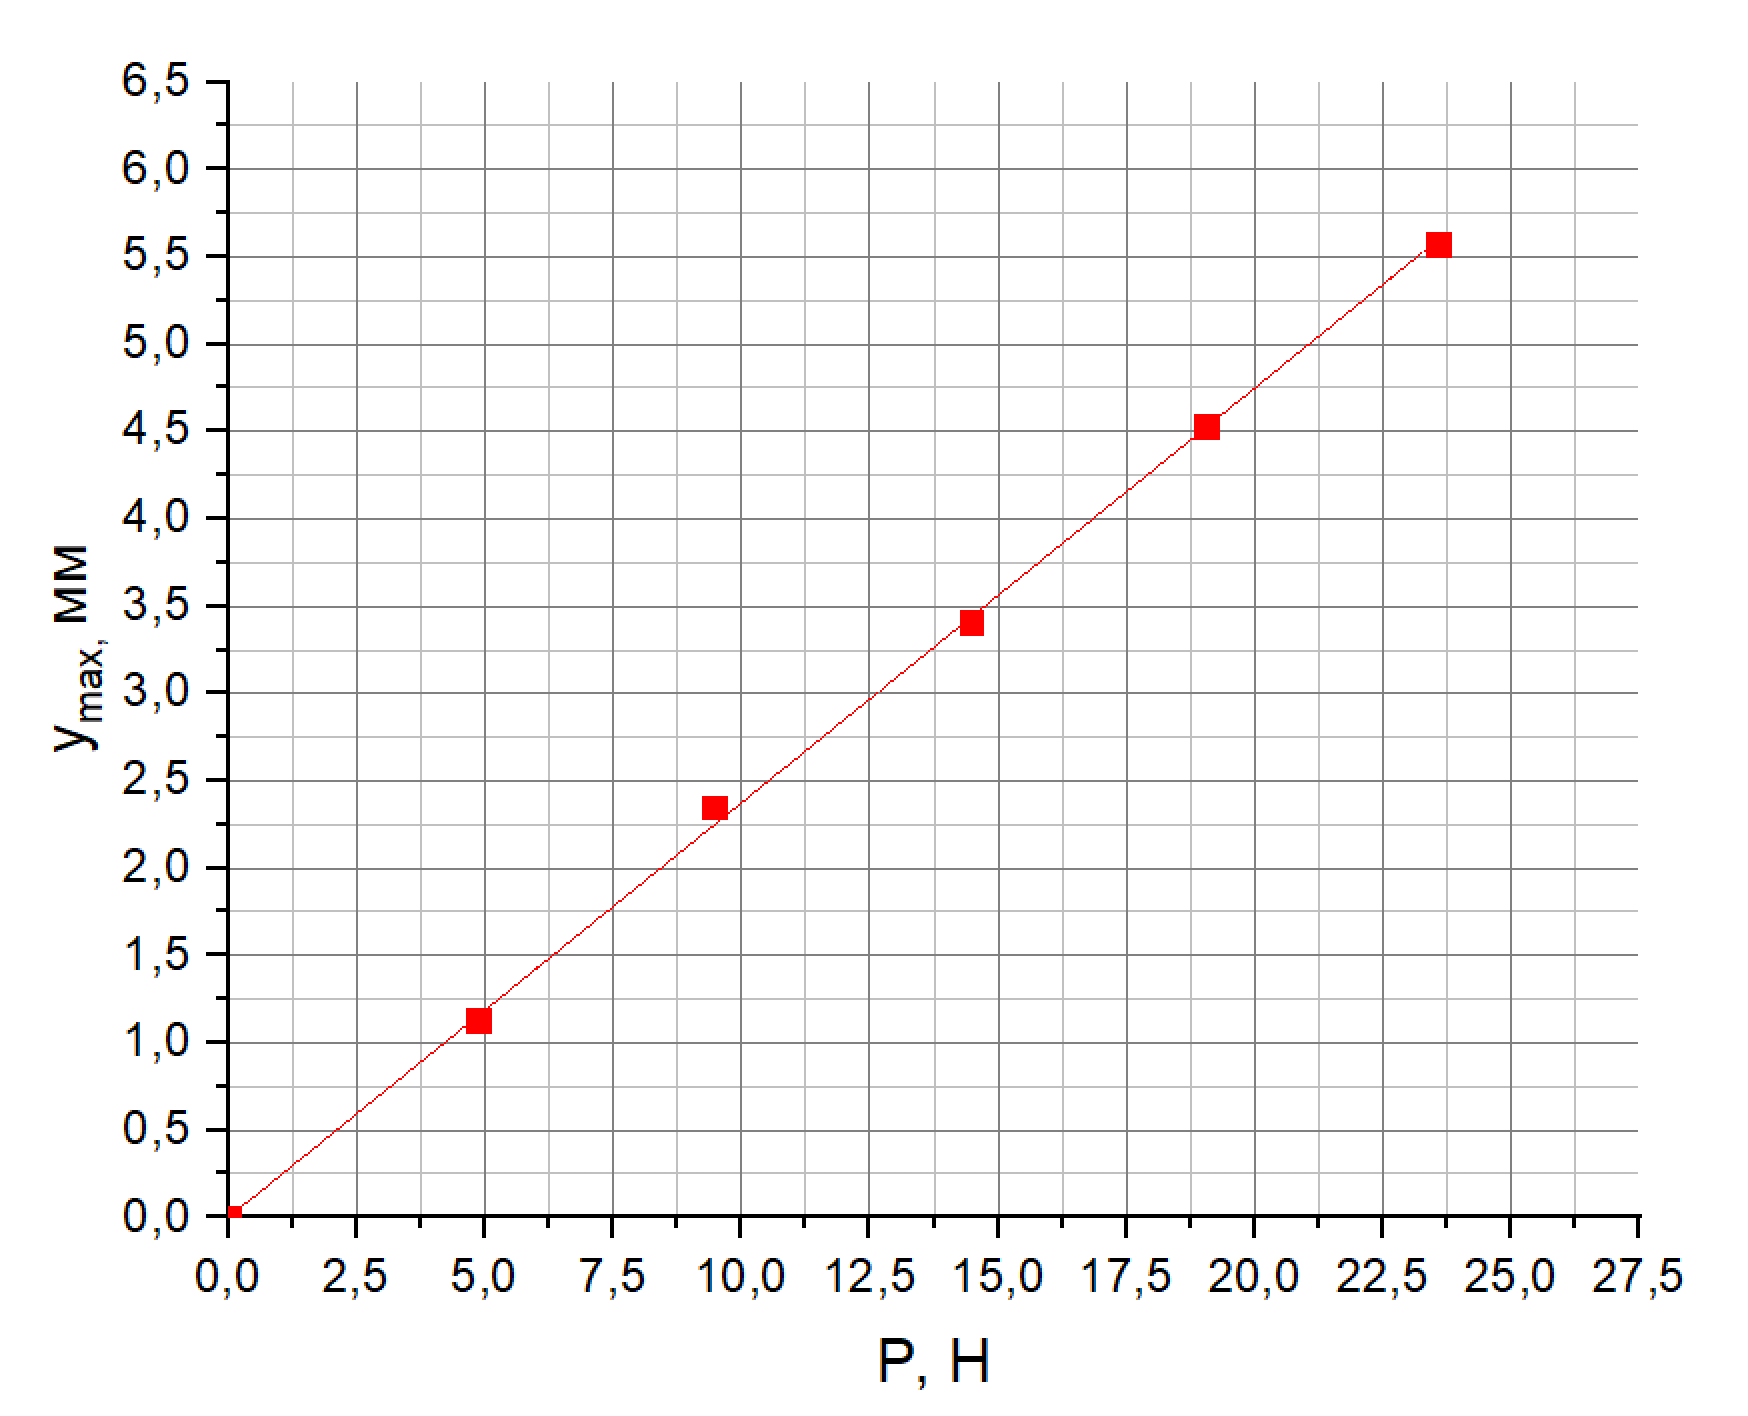
\includegraphics[scale=0.32]{6}
\caption{Зависимость перемещения середины стержня при нагрузке металлической балки}
\end{figure}

\newpage
\begin{figure}[h]
\centering
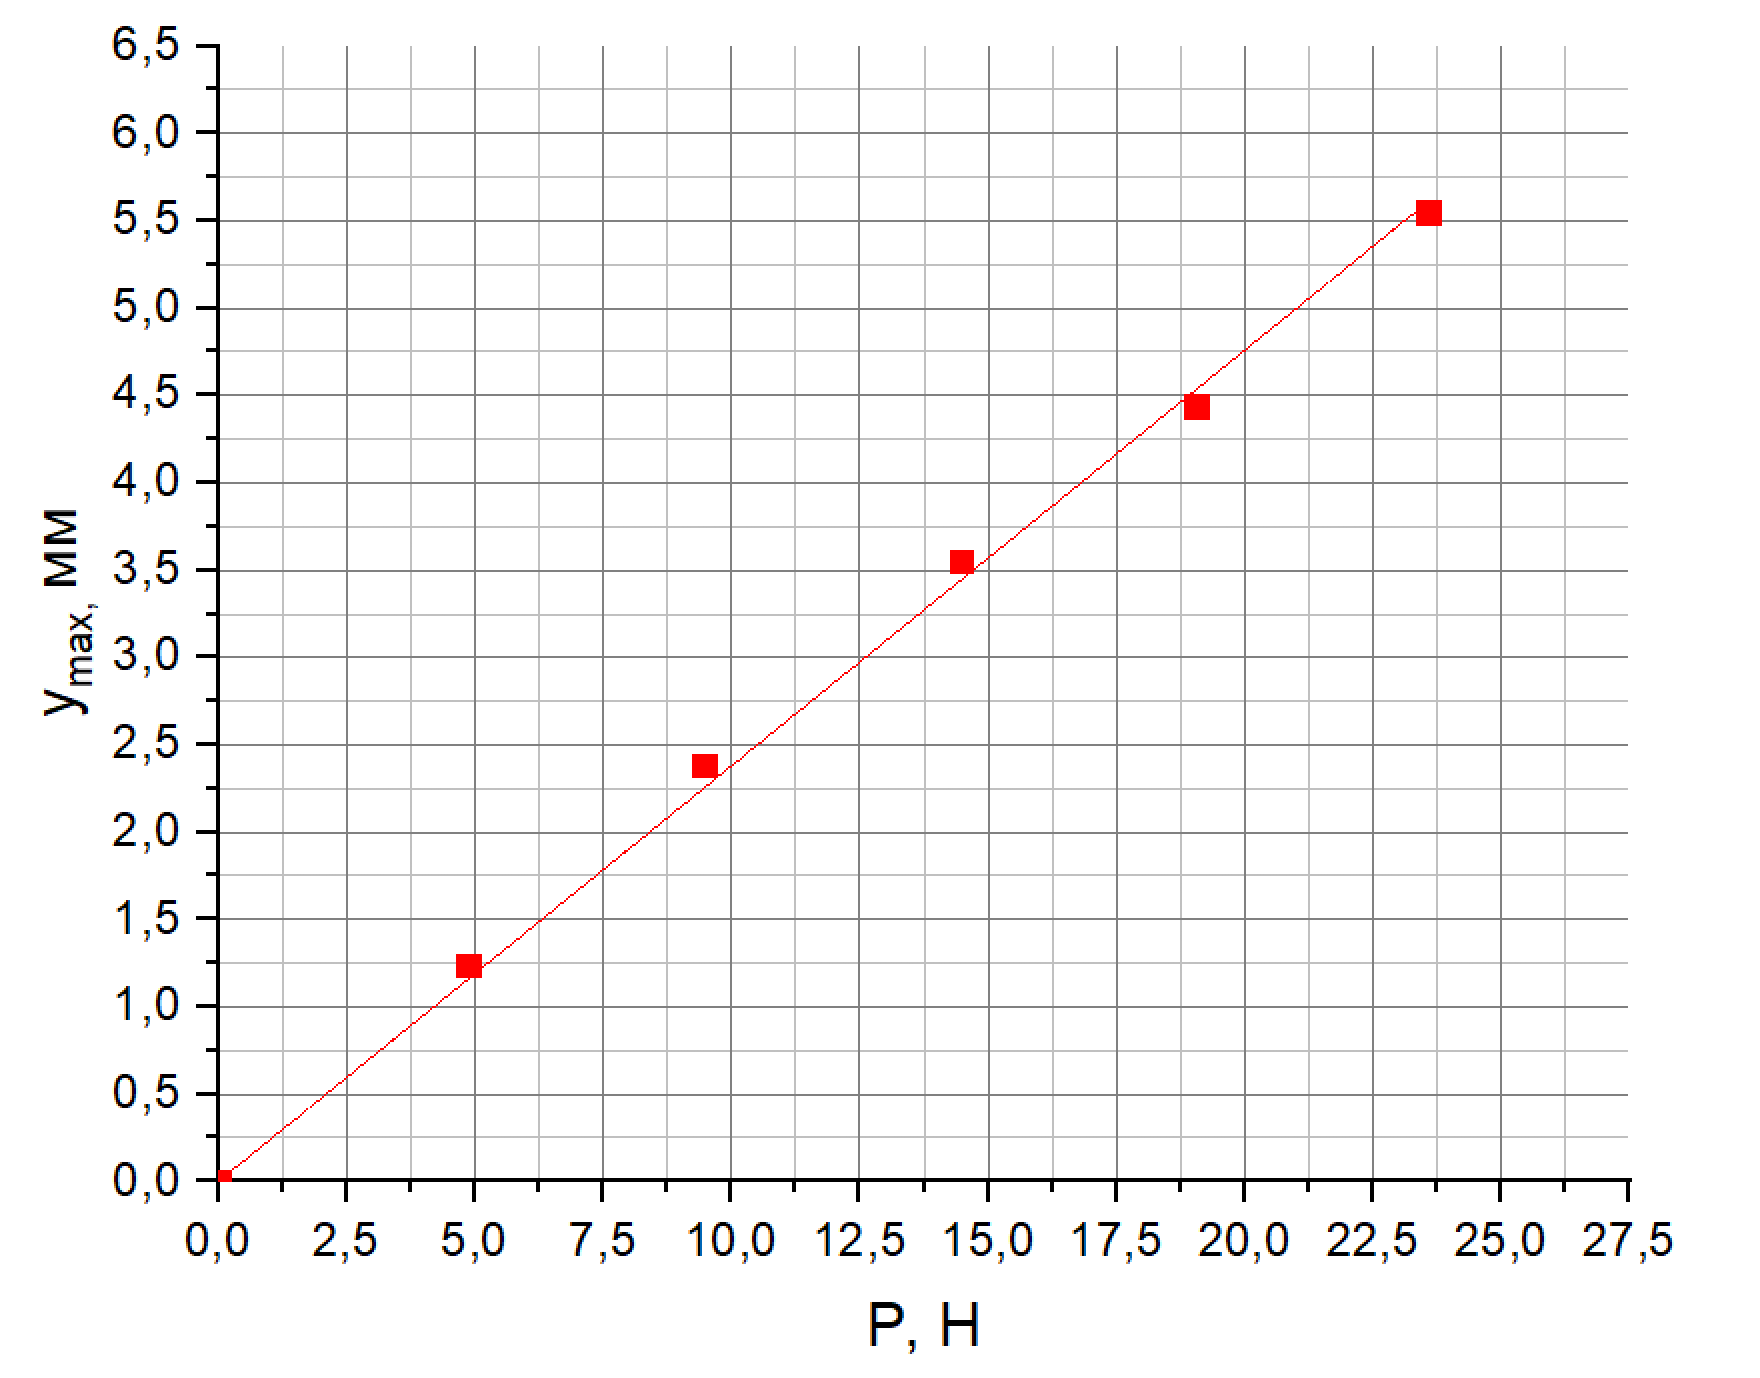
\includegraphics[scale=0.32]{7}
\caption{Зависимость перемещения середины стержня при pазгрузке металлической балки}
\end{figure}
\begin{figure}[!h]
\centering
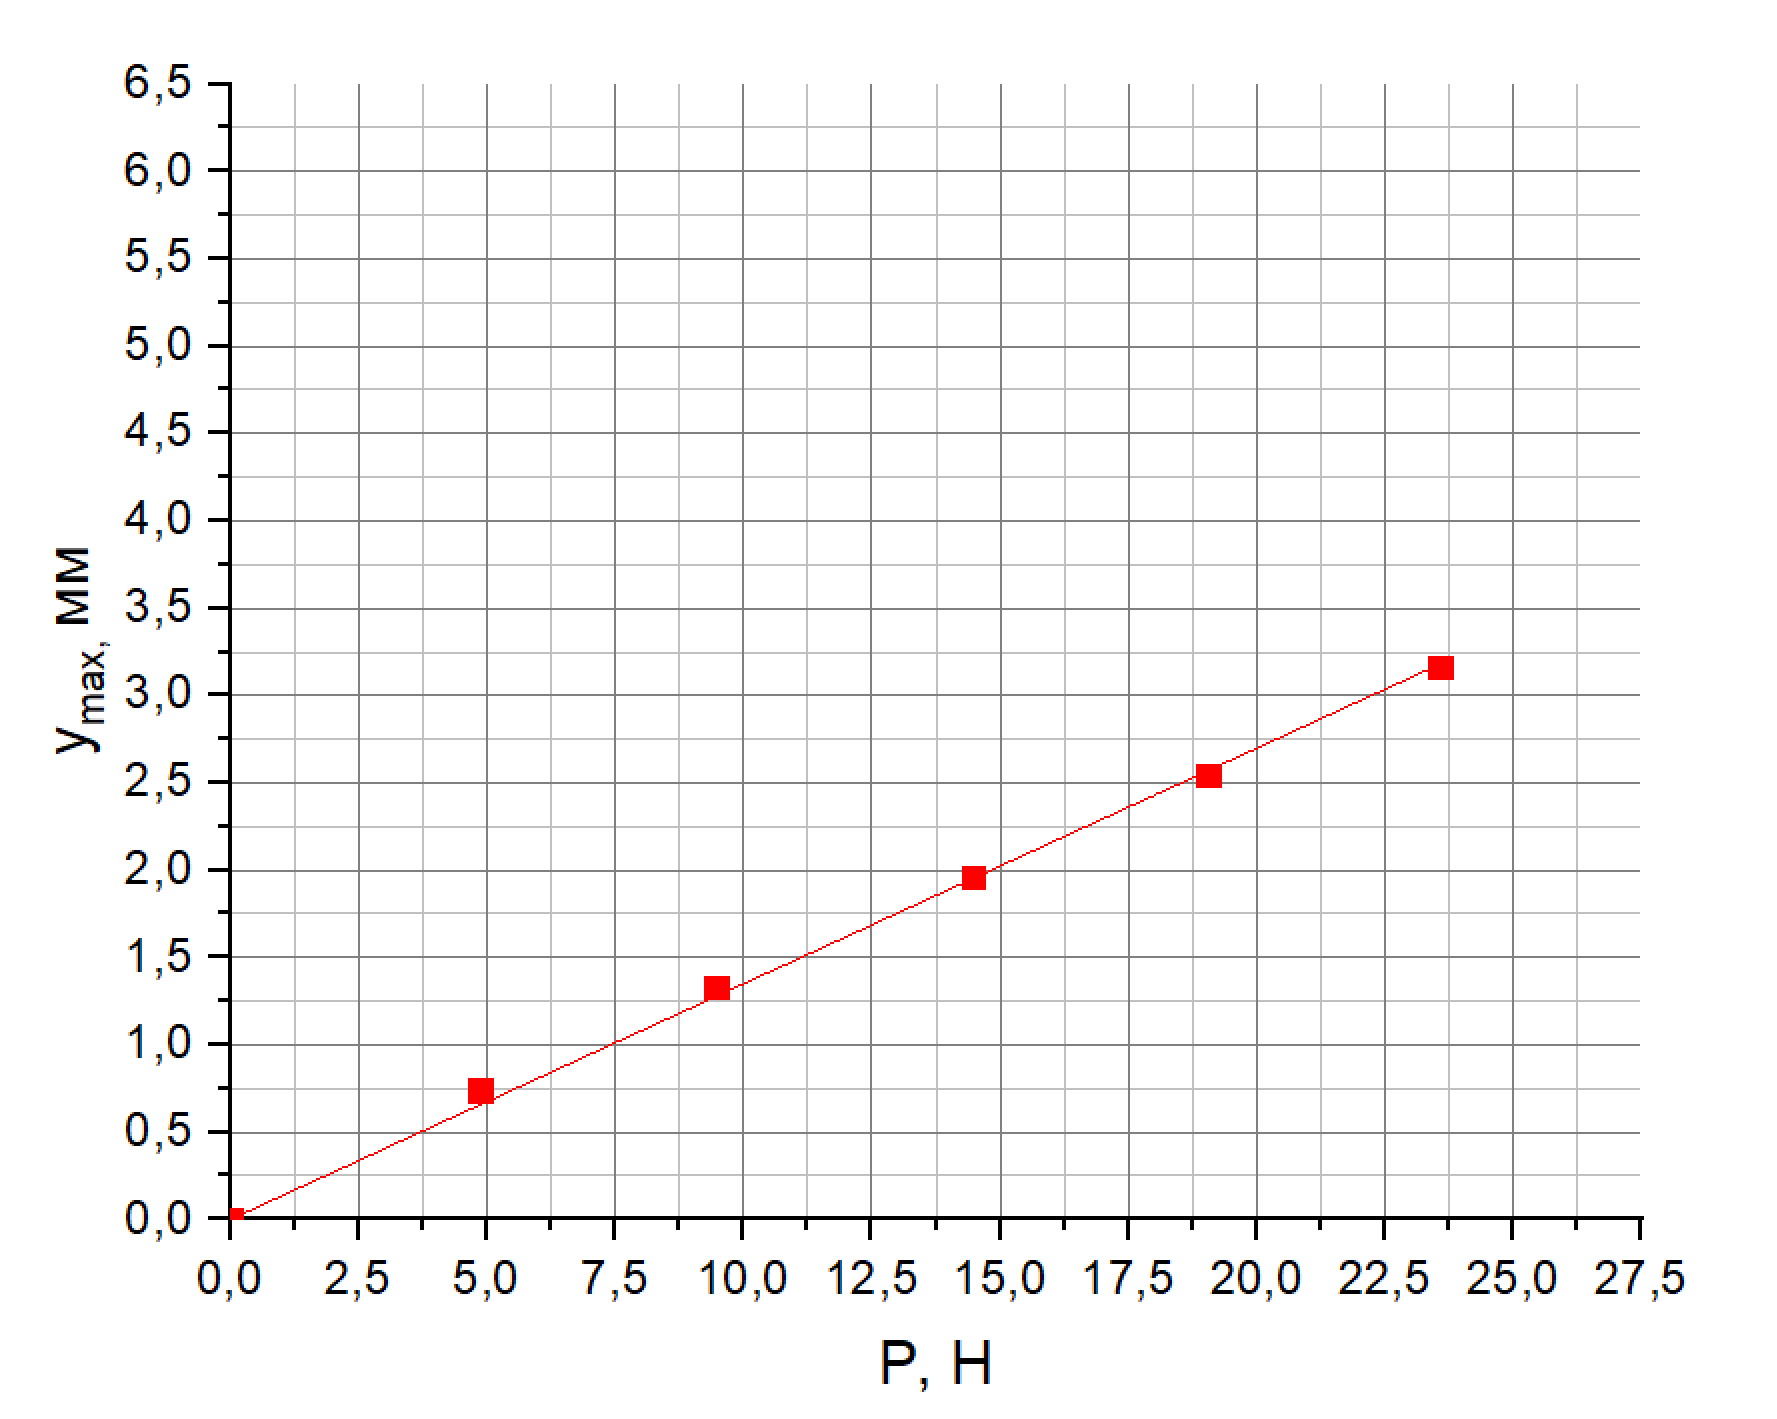
\includegraphics[scale=0.32]{8}
\caption{Зависимость перемещения середины стержня при нагрузке первой деревянной балки}
\end{figure}
\newpage
\begin{figure}[h]
\centering
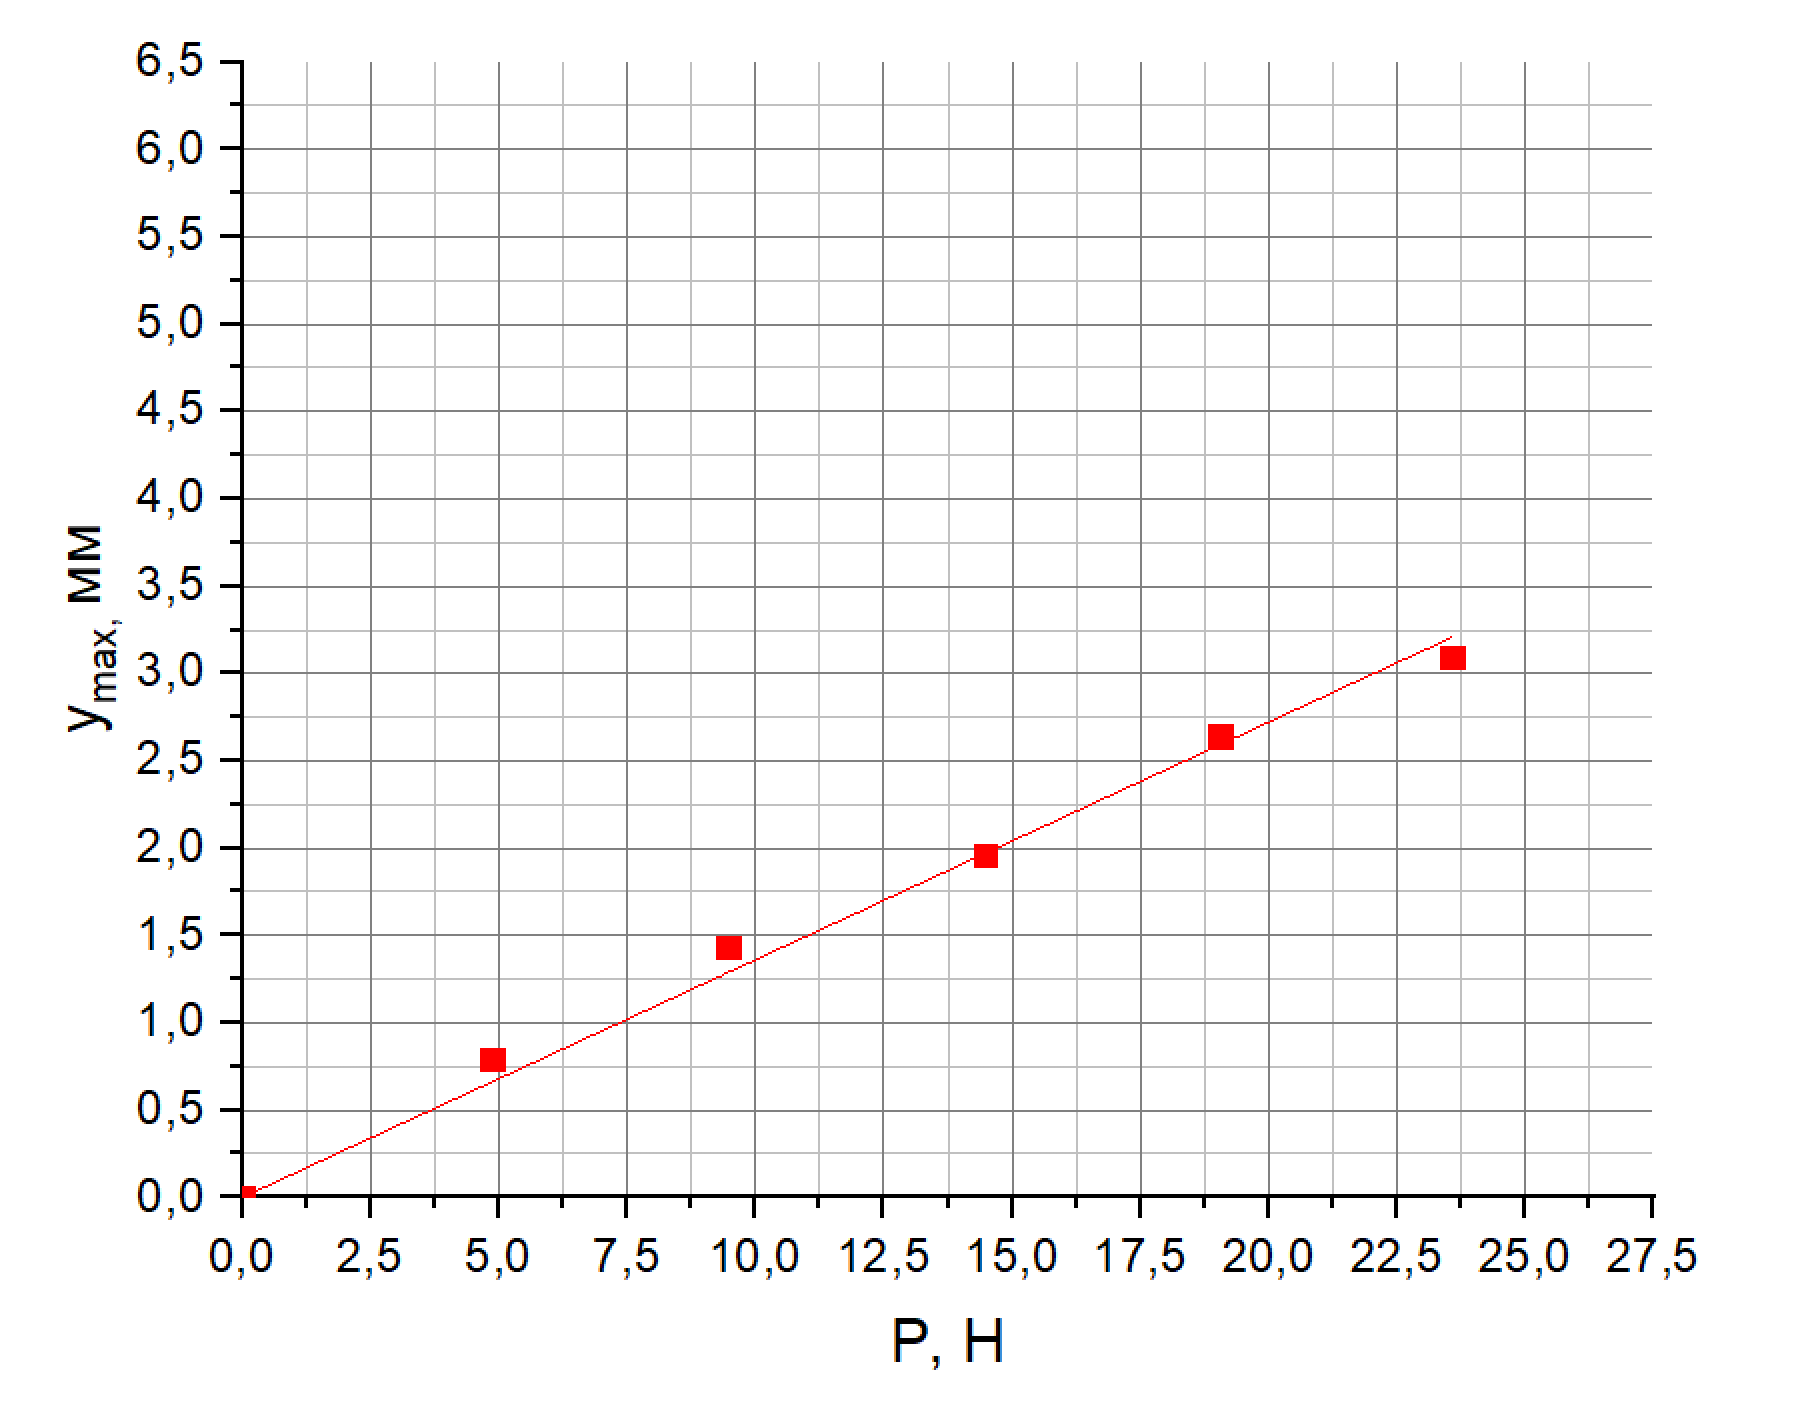
\includegraphics[scale=0.32]{9}
\caption{Зависимость перемещения середины стержня при разгрузке первой деревянной балки}
\end{figure}
\begin{figure}[!h]
\centering
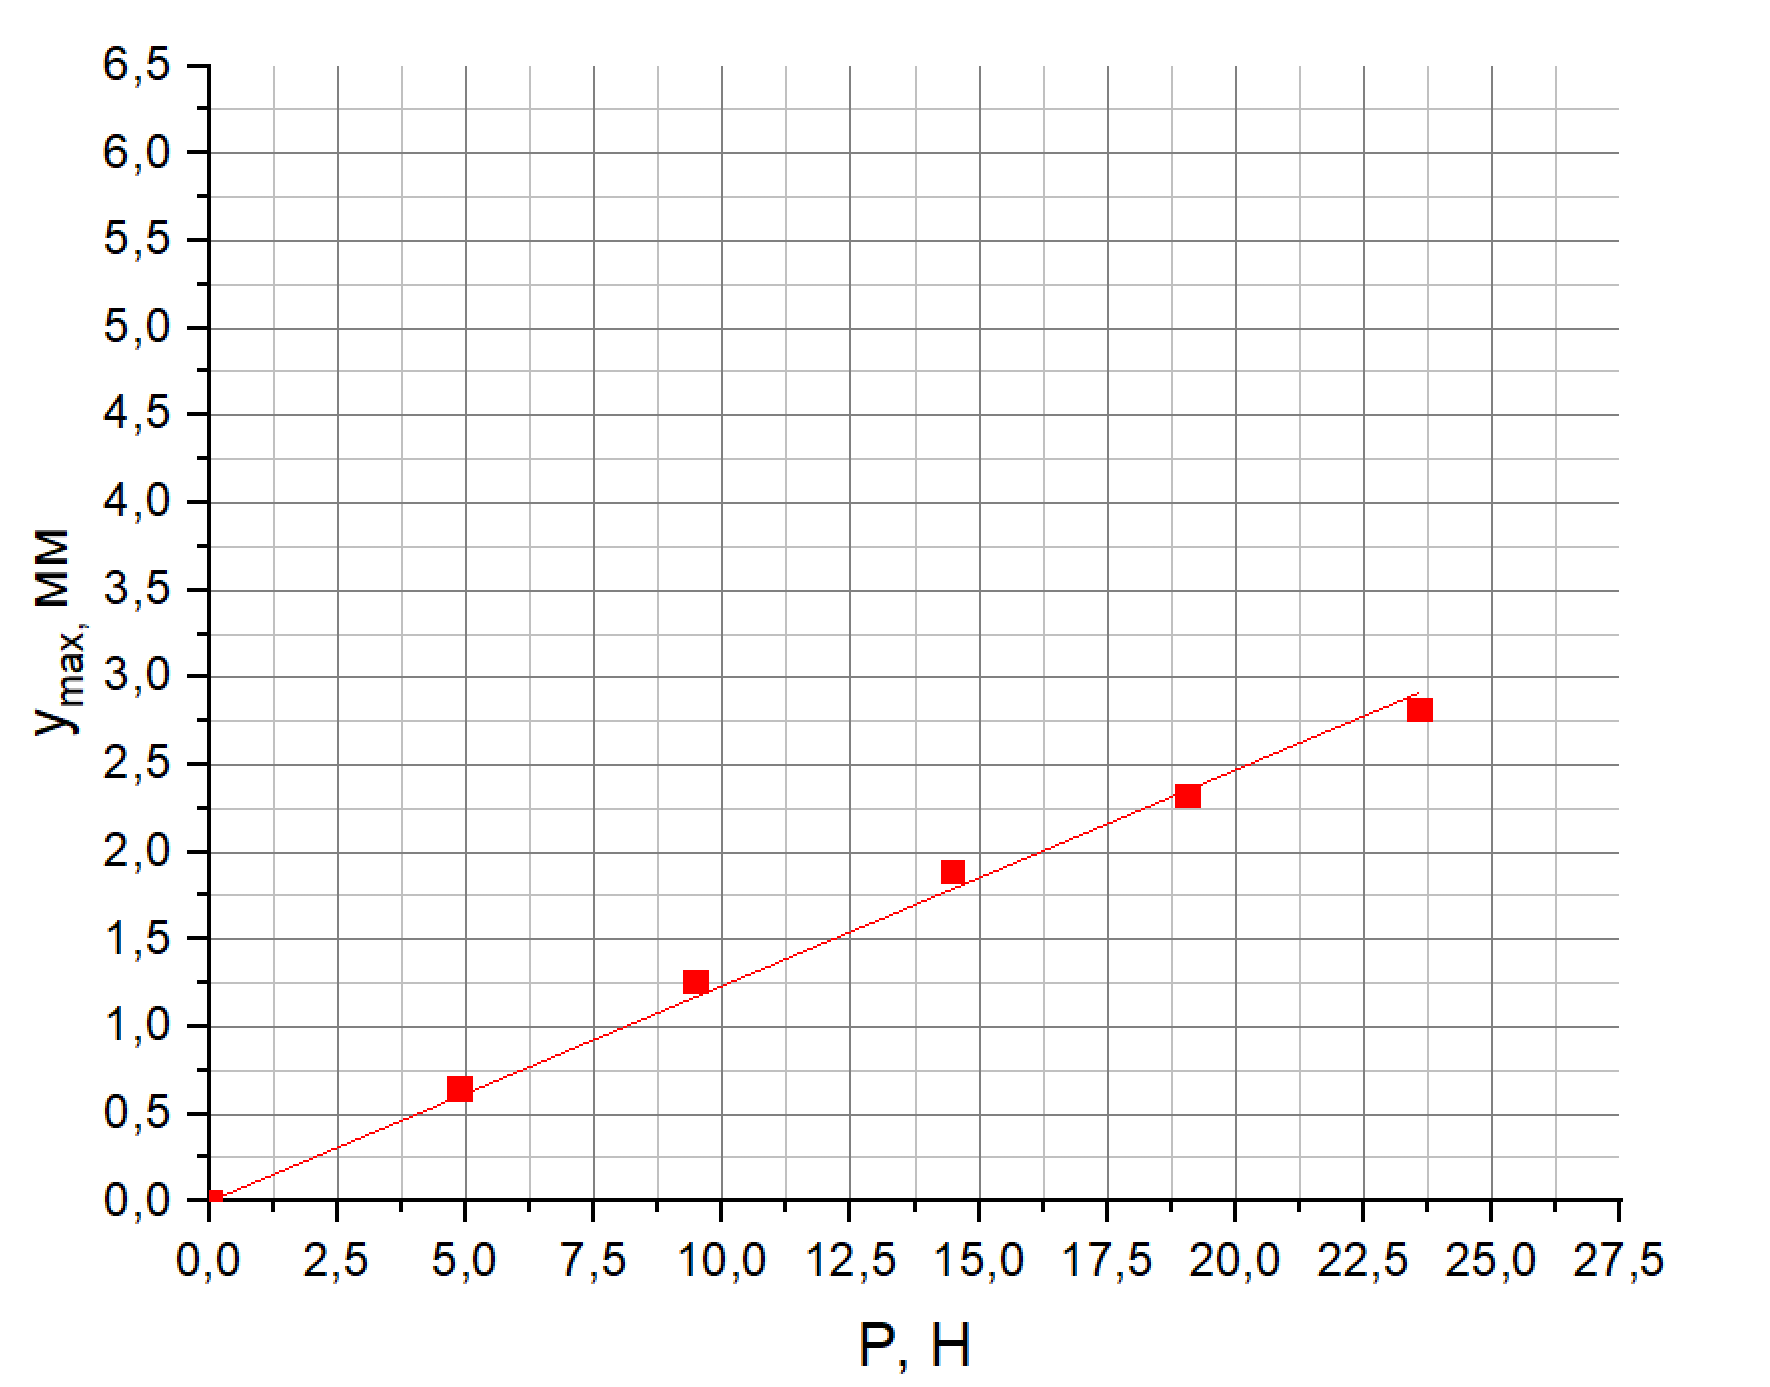
\includegraphics[scale=0.32]{10}
\caption{Зависимость перемещения середины стержня при нагрузке второй деревянной балки}
\end{figure}
\newpage
\begin{figure}[!h]
\centering
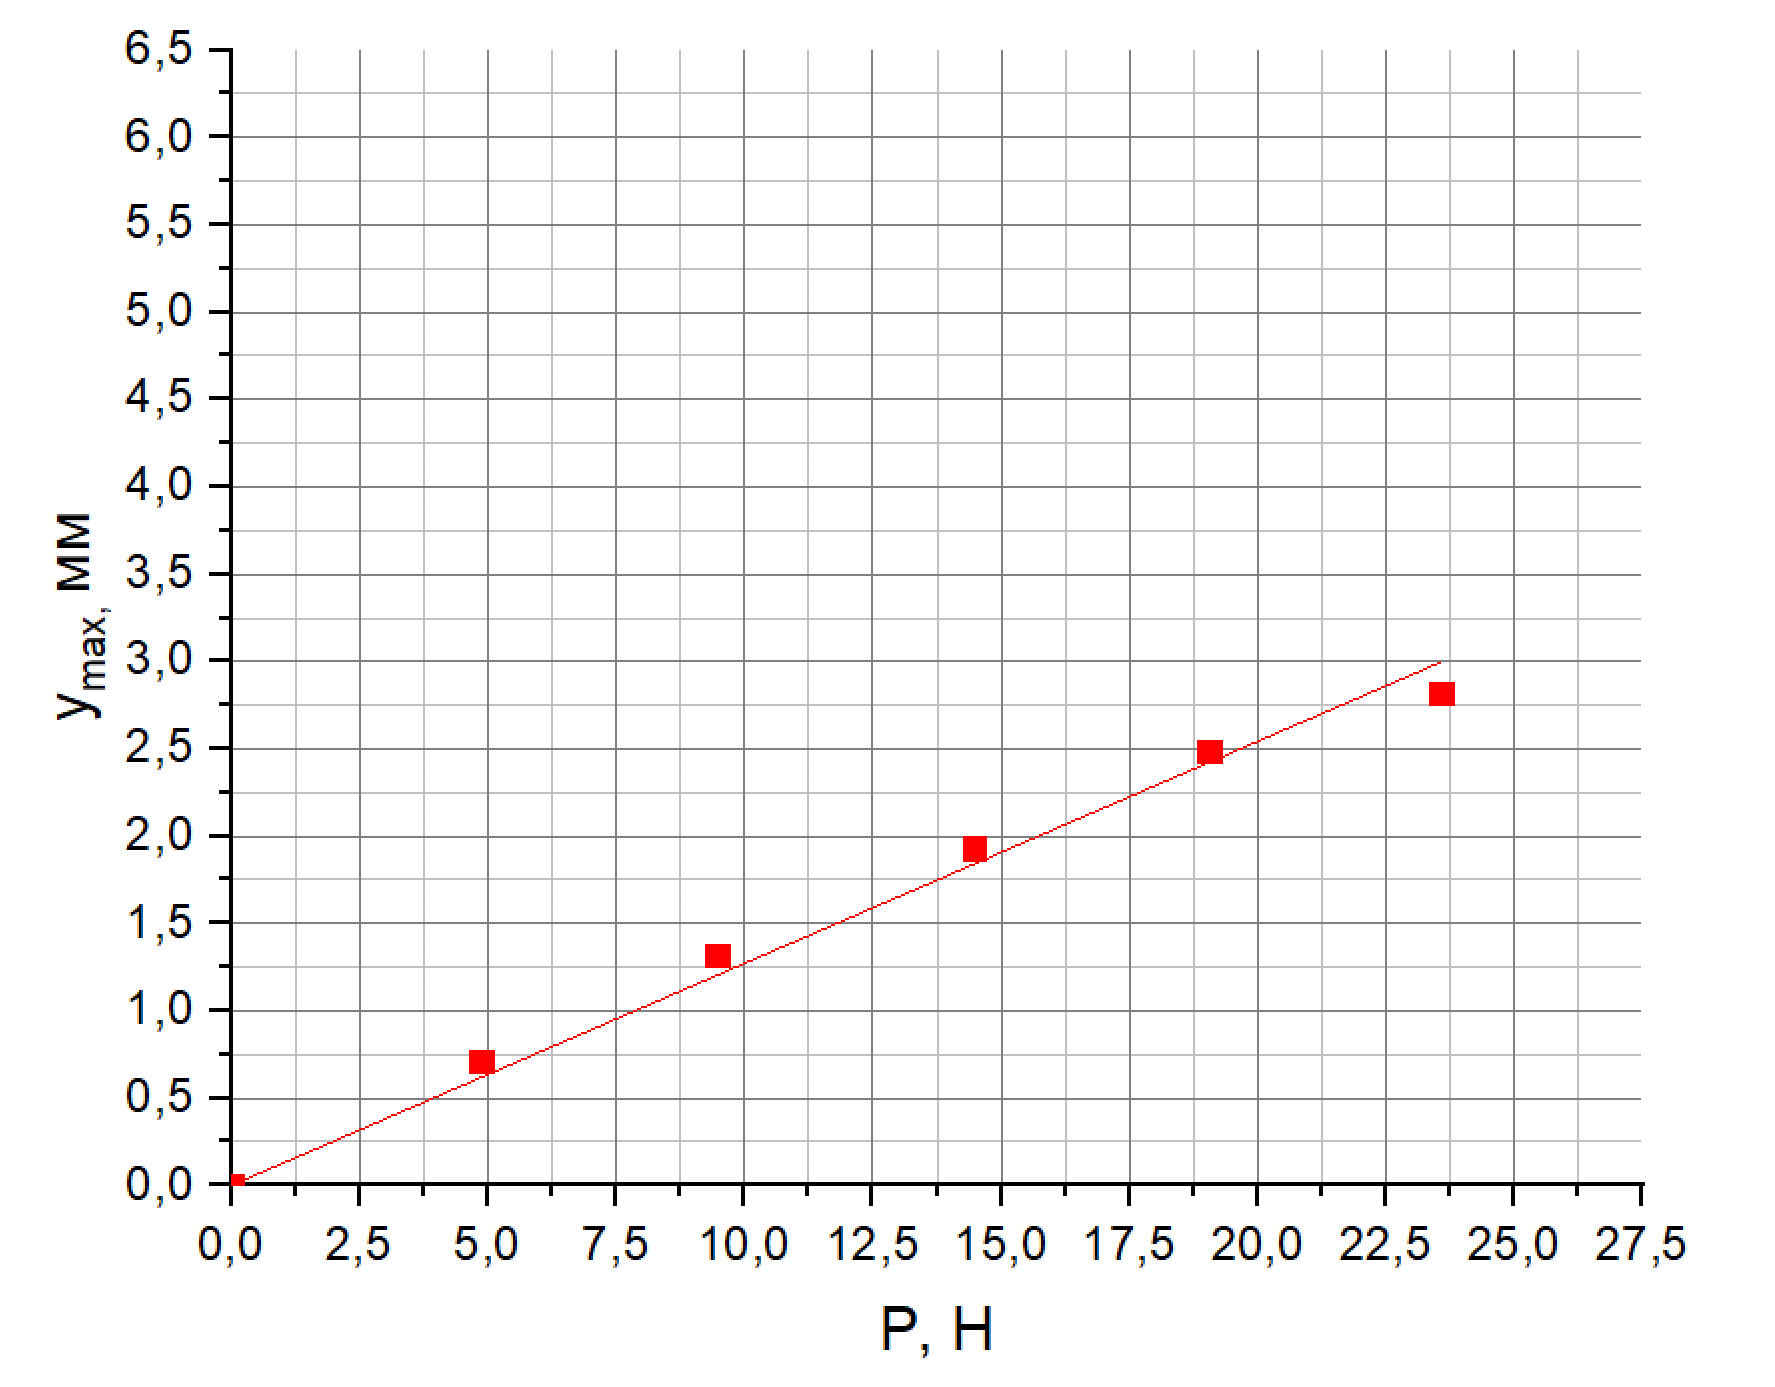
\includegraphics[scale=0.32]{11}
\caption{Зависимость перемещения середины стержня при разгрузке второй деревянной балки}
\end{figure}
Переворачиваем балки таким образом, чтобы при напряжении она изгибалась в противоположную сторону и повторяем измерения. Результаты заносим в Таблицы 8, 9, 10.
\begin{table}[h]
\centering
\begin{tabular}{|c|c|c|c|c|c|}
\hline
$m, \text{г}$   & $P,  H$    & $x_{max}, \text{мм}$ &  $y_{max}, \text{мм}$    & $x'_{max}, \text{мм}$ &    $y'_{max}, \text{мм}$  \\ \hline
0      & 0      & 5,87 & 0    & 5,85 & 0    \\ \hline
497,3  & 0,487  & 4,69 & 1,18 & 4,63 & 1,22 \\ \hline
965,2  & 0,946  & 3,57 & 2,3  & 3,48 & 2,37 \\ \hline
1476,2 & 1,447 & 2,25 & 3,62 & 2,24 & 3,61 \\ \hline
1943,8 & 1,905 & 1,15 & 4,72 & 1,11 & 4,74 \\ \hline
2405,6 & 2,357 & 0,17 & 5,7  & 0,17 & 5,68 \\ \hline
\end{tabular}
\caption{Зависимость стрелы прогиба от величины нагрузки для металлической балки (перевернутой)}
\end{table}
\begin{table}[!h]
\centering
\begin{tabular}{|c|c|c|c|c|c|}
\hline
$m, \text{г}$   & $P,  H$    & $x_{max}, \text{мм}$ &  $y_{max}, \text{мм}$    & $x'_{max}, \text{мм}$ &    $y'_{max}, \text{мм}$  \\ \hline
0      & 0      & 6,52 & 0    & 6,13 & 0    \\ \hline
497,3  & 0,487  & 5,85 & 0,67 & 5,42 & 0,71 \\ \hline
965,2  & 0,946  & 4,97 & 1,55 & 4,72 & 1,41 \\ \hline
1476,2 & 1,447 & 4,15 & 2,37 & 3,99 & 2,14 \\ \hline
1943,8 & 1,905 & 3,35 & 3,17 & 3,35 & 2,78 \\ \hline
2405,6 & 2,457 & 2,64 & 3,88 & 2,64 & 3,49 \\ \hline
\end{tabular}
\caption{Зависимость стрелы прогиба от величины нагрузки для первой деревянной балки(перевернутой)}
\end{table}
\newpage
\begin{table}[h]
\centering
\begin{tabular}{|c|c|c|c|c|c|}
\hline
$m, \text{г}$   & $P,  H$    & $x_{max}, \text{мм}$ &  $y_{max}, \text{мм}$    & $x'_{max}, \text{мм}$ &    $y'_{max}, \text{мм}$  \\ \hline
0      & 0      & 4,34 & 0    & 4,31 & 0    \\ \hline
497,3  & 0,487  & 3,69 & 0,65 & 3,6  & 0,71 \\ \hline
965,2  & 0,946  & 3,1  & 1,24 & 3,01 & 1,3  \\ \hline
1476,2 & 1,447 & 2,44 & 1,9  & 2,38 & 1,93 \\ \hline
1943,8 & 1,905 & 1,96 & 2,38 & 1,9  & 2,41 \\ \hline
2405,6 & 2,457 & 1,53 & 2,81 & 1,53 & 2,78 \\ \hline
\end{tabular}
\caption{Зависимость стрелы прогиба от величины нагрузки для второй деревянной балки(перевернутой)}
\end{table}

Сместим призму Д на 2-3мм от точки, принятой за середину балки и измерим стрелу прогиба. Результат занесем в Таблицу 11.
\begin{table}[!h]
\centering
\begin{tabular}{|c|c|c|c|c|c|}
\hline
$m, \text{г}$   & $P,  H$    & $x_{max}, \text{мм}$ &  $y_{max}, \text{мм}$    & $x'_{max}, \text{мм}$ &    $y'_{max}, \text{мм}$  \\ \hline
0      & 0        & 7,8  & 0    & 7,76 & 0    \\ \hline
497,3  & 0,487354  & 7,19 & 0,61 & 7,1  & 0,66 \\ \hline
965,2  & 0,945896  & 6,63 & 1,17 & 6,48 & 1,28 \\ \hline
1476,2 & 1,446676 & 5,9  & 1,9  & 5,78 & 1,98 \\ \hline
1943,8 & 1,904924 & 5,29 & 2,51 & 5,21 & 2,55 \\ \hline
2405,6 & 2,357488 & 4,86 & 2,94 & 4,86 & 2,9  \\ \hline
\end{tabular}
\caption{Зависимость стрелы прогиба от величины нагрузки для первой деревянной балки(смещенной на 2-3мм)}
\end{table}

Посчитаем модуль Юнга с помощью графиков (Рис. 5-10) и формулы (20)
\[E_{\text{мет}} = (96,1\pm1,1)\text{ГПа}\]
\[E_{\text{дер}_1} = (9,5\pm0,9)\text{ГПa}\]
\[E_{\text{дер}_2} = (11,0\pm0,5)\text{ГПa}\]
\section{Обсуждение результатов и выводы}
В работе был определен модуль Юнга с помщью графика зависимости между удлинением проволки и нагрузки на нее для одноосного растяжения проволоки:
\[E = (167\pm11)\text{ГПа}\]
Значение Модулю Юнга для стали, полученное в эксперименте соответсвует табличному.

Также был  определен модуль Юнга с помщью зависимостм стрелы прогиба от величины нагрузки на балку из исследумего материала.
\[E_{\text{мет}} = (96,1\pm1,1)\text{ГПа}\]
Значение Модулю Юнга для латуни, полученное в эксперименте соответсвует табличному.
\[E_{\text{дер}_1} = (9,5\pm0,9)\text{ГПa}\]
\[E_{\text{дер}_2} = (11,0\pm0,5)\text{ГПa}\]
Значение Модулю Юнга для дерева, полученное в эксперименте соответсвует табличному (предположительно балка была из сосны).

Из сравнения результатов в Таблицах 5, 6, 7 с результатами в Таблицах 8, 9, 10 следует, что при перевороте металлической балки смещение середины балки при соответсующих нагрузках почти не изменяется; при перевороте деревянных баллок изменения более заметны в виду формы балки. 

Из сравнения результатов в Таблце 6 с результатами в Таблице 11 следует, что при смещении балки на 2-3 мм пермещения середин балок для одинаковых нагрузок приблизительно равны.
\end{document}